\subsection{Machine Learning}

El \textit{Machine Learning} (aprendizaje automático) es una rama de la inteligencia artificial que permite a los sistemas aprender y mejorar automáticamente a partir de la experiencia, sin ser programados explícitamente para cada tarea. Utiliza algoritmos que identifican patrones en grandes volúmenes de datos y toman decisiones o realizan predicciones basadas en esos patrones.

En el contexto de los Sistemas de Detección de Intrusos (IDS), el \textit{Machine Learning} se emplea para analizar el tráfico de red y detectar comportamientos anómalos o maliciosos de manera más eficiente y precisa que los métodos tradicionales basados en firmas. Además, la relación con la \textit{Green AI} surge porque el uso de técnicas de aprendizaje automático más eficientes puede reducir el consumo energético, promoviendo soluciones más sostenibles.

\subsubsection{Random Forest (RF)}

\textbf{Random Forest} es un algoritmo de aprendizaje supervisado basado en un ensamblado de árboles de decisión entrenados de forma independiente. El modelo construye múltiples árboles utilizando distintas muestras del conjunto de entrenamiento obtenidas mediante \textit{bootstrap sampling}, así como subconjuntos aleatorios de características en cada división. La predicción final se obtiene combinando las salidas de todos los árboles, habitualmente mediante votación mayoritaria en tareas de clasificación.

A diferencia de los métodos de \textit{boosting}, como XGBoost, los árboles que componen un Random Forest no se entrenan de manera secuencial ni dependen unos de otros. Cada árbol aprende de forma autónoma a partir de una vista ligeramente distinta de los datos, lo que permite reducir la varianza del modelo y mejorar su robustez frente al ruido y al sobreajuste. Esta independencia entre árboles hace que Random Forest sea especialmente estable y fiable como modelo base en problemas de detección de intrusiones.

Desde el punto de vista de la inferencia, Random Forest presenta una latencia muy reducida, ya que la predicción consiste únicamente en recorrer un número limitado de árboles poco profundos y agregar sus decisiones. Además, al no requerir cálculos iterativos complejos ni funciones de activación costosas, su consumo computacional durante la fase de operación es bajo, lo que lo convierte en una opción adecuada para despliegues en entornos con recursos limitados.

En el contexto de \textit{Green AI}, Random Forest destaca por ofrecer un excelente equilibrio entre rendimiento y eficiencia energética. Aunque el entrenamiento puede ser más costoso que el de un único árbol de decisión, este proceso se realiza de forma puntual y fuera de línea. En contraste, la fase de inferencia es altamente eficiente, lo que resulta especialmente relevante en sistemas de detección de intrusiones que deben operar de forma continua en tiempo real.

\begin{table}[H]
    \centering
    \caption{Principales hiperparámetros de Random Forest y su significado.}
    \label{tab:rf_hyperparams}
    \begin{tabular}{ll}
        \toprule
        \textbf{Hiperparámetro} & \textbf{Significado} \\
        \midrule
        \texttt{n\_estimators} & Número de árboles en el bosque \\
        \texttt{max\_depth} & Profundidad máxima de cada árbol \\
        \texttt{min\_samples\_split} & Mínimo de muestras para dividir un nodo \\
        \texttt{min\_samples\_leaf} & Mínimo de muestras en una hoja \\
        \texttt{max\_features} & Número de características consideradas en cada división \\
        \texttt{bootstrap} & Si se usan muestras con reemplazo para entrenar cada árbol \\
        \texttt{criterion} & Función para medir la calidad de una división (por ejemplo, \textit{gini} o \textit{entropy}) \\
        \bottomrule
    \end{tabular}
\end{table}

\begin{figure}[H]
    \centering
    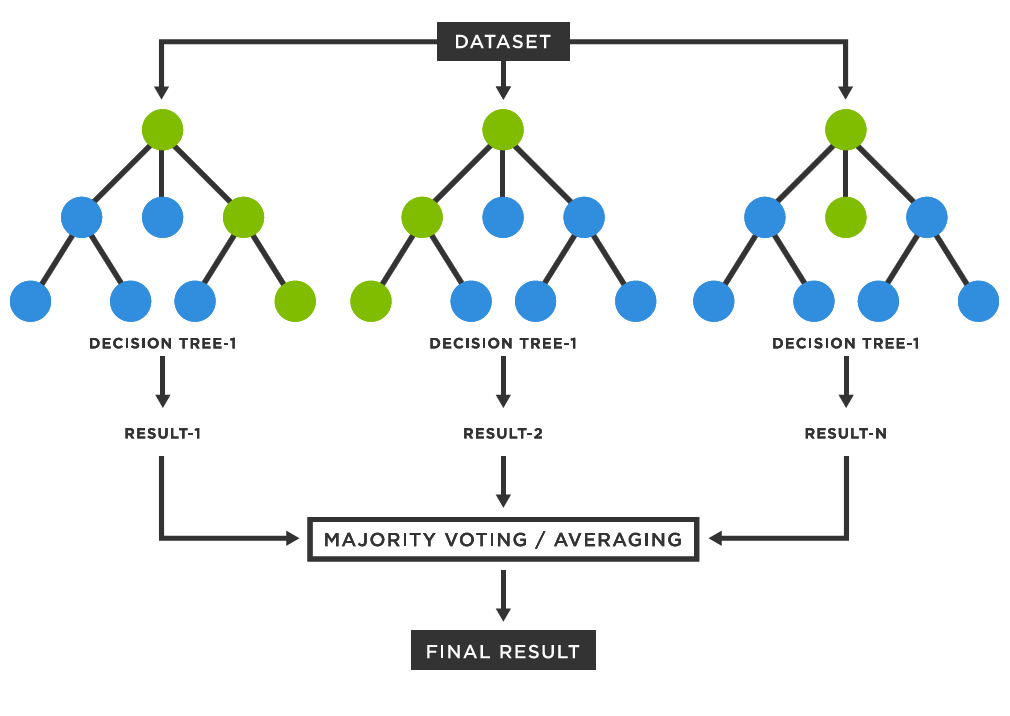
\includegraphics[width=0.7\textwidth]{images/random_forest.png}
    \caption{Esquema representativo del funcionamiento de Random Forest.}
    \label{fig:randomforest}
\end{figure}

\subsubsection{Extreme Gradient Boosting (XGBoost)}

\textbf{XGBoost} (\textit{Extreme Gradient Boosting}) es un algoritmo de aprendizaje supervisado basado en árboles de decisión que implementa de forma altamente optimizada el principio de \textit{gradient boosting}. A diferencia de otros métodos basados en ensamblados de árboles, XGBoost construye el modelo de manera secuencial, añadiendo nuevos árboles que se centran en corregir los errores cometidos por los árboles previamente entrenados. Este proceso se basa en la optimización iterativa de una función objetivo que combina el error de clasificación con términos explícitos de regularización, lo que permite controlar la complejidad del modelo y reducir el sobreajuste.

En cada iteración, XGBoost utiliza información de primer y segundo orden del gradiente de la función de pérdida para determinar la estructura óptima de los árboles, lo que le permite capturar relaciones no lineales complejas e interacciones entre características de forma eficiente. Estas propiedades lo convierten en una opción especialmente adecuada para la detección de intrusiones en conjuntos de datos tabulares, donde los patrones maliciosos suelen manifestarse a través de combinaciones no triviales de múltiples variables.

En XGBoost, la predicción final del modelo no corresponde a la salida de un único árbol de decisión, sino que se obtiene como la combinación aditiva de las salidas de todos los árboles entrenados. Cada árbol aporta una contribución parcial a la predicción, y el resultado final se calcula sumando dichas contribuciones.
El proceso de entrenamiento es secuencial: cada nuevo árbol se entrena para corregir los errores residuales cometidos por el conjunto de árboles previamente construidos. Como consecuencia, el último árbol no contiene una decisión completa por sí mismo, sino que únicamente modela aquellos patrones que aún no han sido correctamente capturados por los árboles anteriores, actuando como un ajuste fino del modelo global.
De este modo, XGBoost se centra en la reducción del sesgo, lo que suele traducirse en un mayor rendimiento predictivo cuando se dispone de un número limitado de características relevantes.

En el contexto de este trabajo, la elección de XGBoost resulta especialmente adecuada al considerar criterios de eficiencia computacional y sostenibilidad, en línea con los principios de \textit{Green AI}. Aunque el proceso de entrenamiento de XGBoost puede ser más costoso que el de otros modelos clásicos, este se realiza de forma puntual y fuera de línea. En cambio, la fase de inferencia presenta una latencia muy reducida, ya que únicamente requiere recorrer un número limitado de árboles poco profundos, lo que lo hace compatible con despliegues en entornos \textit{edge} e IoT. Por tanto, XGBoost ofrece un equilibrio muy favorable entre rendimiento y coste computacional, permitiendo alcanzar altas tasas de detección sin incurrir en un consumo energético elevado durante la operación del sistema IDS.

\begin{table}[H]
    \centering
    \caption{Principales hiperparámetros de XGBoost y su significado.}
    \label{tab:xgboost_hyperparams}
    \begin{tabular}{ll}
        \toprule
        \textbf{Hiperparámetro} & \textbf{Significado} \\
        \midrule
        \texttt{n\_estimators} & Número de árboles a construir \\
        \texttt{max\_depth} & Profundidad máxima de cada árbol \\
        \texttt{learning\_rate} & Tasa de aprendizaje (contribución de cada árbol) \\
        \texttt{subsample} & Proporción de muestras usadas en cada iteración \\
        \texttt{colsample\_bytree} & Proporción de características usadas por árbol \\
        \texttt{gamma} & Mínima reducción de pérdida para dividir un nodo \\
        \texttt{reg\_alpha} & Término de regularización L1 \\
        \texttt{reg\_lambda} & Término de regularización L2 \\
        \texttt{objective} & Función objetivo a optimizar (por ejemplo, \textit{binary:logistic}) \\
        \bottomrule
    \end{tabular}
\end{table}

\begin{figure}[H]
    \centering
    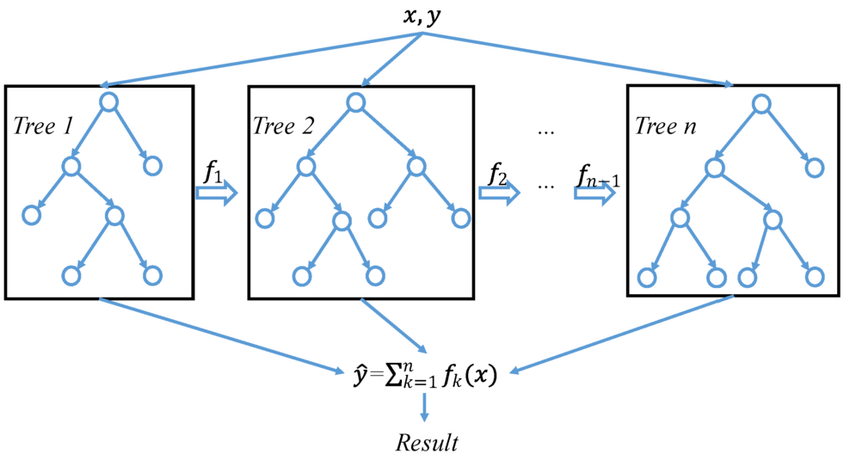
\includegraphics[width=0.7\textwidth]{images/xg_boost.png}
    \caption{Esquema representativo del funcionamiento de XGBoost.}
    \label{fig:xgboost}
\end{figure}

\subsubsection{Support Vector Machine (SVM)}

\textbf{Support Vector Machines} (SVM) es un algoritmo de aprendizaje supervisado cuyo objetivo principal es encontrar una frontera de decisión que separe de forma óptima las distintas clases en el espacio de características. En su formulación básica, SVM busca el hiperplano que maximiza el margen entre las muestras de distintas clases, utilizando únicamente un subconjunto de los datos denominado \textit{vectores soporte}. Esta propiedad permite construir modelos robustos frente al ruido y con buena capacidad de generalización.

Una de las principales fortalezas de las SVM es el uso de \textit{kernels}, que permiten proyectar los datos originales a espacios de mayor dimensionalidad sin realizar explícitamente dicha transformación. Gracias a este mecanismo, SVM puede modelar fronteras de decisión no lineales incluso cuando los datos no son separables linealmente en el espacio original. Entre los kernels más utilizados se encuentran:

\begin{itemize}
    \item \textbf{Kernel lineal}: Define una frontera de decisión lineal en el espacio de características original. Es el kernel más simple y el más eficiente desde el punto de vista computacional, lo que lo hace especialmente adecuado para datasets de gran tamaño y para escenarios donde se prioriza la eficiencia.
    
    \item \textbf{Kernel polinómico}: Permite modelar relaciones no lineales mediante funciones polinómicas de distinto grado. Aunque puede capturar interacciones más complejas entre las características, su coste computacional aumenta rápidamente con el grado del polinomio y el tamaño del dataset.
    
    \item \textbf{Kernel radial (RBF)}: Proyecta los datos a un espacio de dimensión infinita, permitiendo separar patrones altamente no lineales. Si bien suele ofrecer un alto rendimiento predictivo, su entrenamiento e inferencia son significativamente más costosos, especialmente en conjuntos de datos de gran tamaño.
\end{itemize}

En el contexto de este trabajo, el uso de SVM se plantea principalmente mediante un \textbf{kernel lineal}, ya que ofrece un compromiso adecuado entre rendimiento y eficiencia computacional. Los kernels no lineales, como el RBF, resultan poco escalables para los volúmenes de datos considerados y presentan un coste energético elevado, lo que los hace menos compatibles con los principios de \textit{Green AI}.

\begin{table}[H]
    \centering
    \caption{Principales hiperparámetros de SVM y su significado.}
    \label{tab:svm_hyperparams}
    \begin{tabular}{ll}
        \toprule
        \textbf{Hiperparámetro} & \textbf{Significado} \\
        \midrule
        \texttt{C} & Parámetro de regularización que controla el equilibrio entre margen y error de clasificación \\
        \texttt{kernel} & Tipo de función kernel utilizada (por ejemplo, \textit{linear}, \textit{poly}, \textit{rbf}) \\
        \texttt{degree} & Grado del polinomio (solo para kernel polinómico) \\
        \texttt{gamma} & Coeficiente para kernels \textit{rbf}, \textit{poly} y \textit{sigmoid} \\
        \texttt{coef0} & Término independiente en kernels \textit{poly} y \textit{sigmoid} \\
        \bottomrule
    \end{tabular}
\end{table}

\begin{figure}[H]
    \centering
    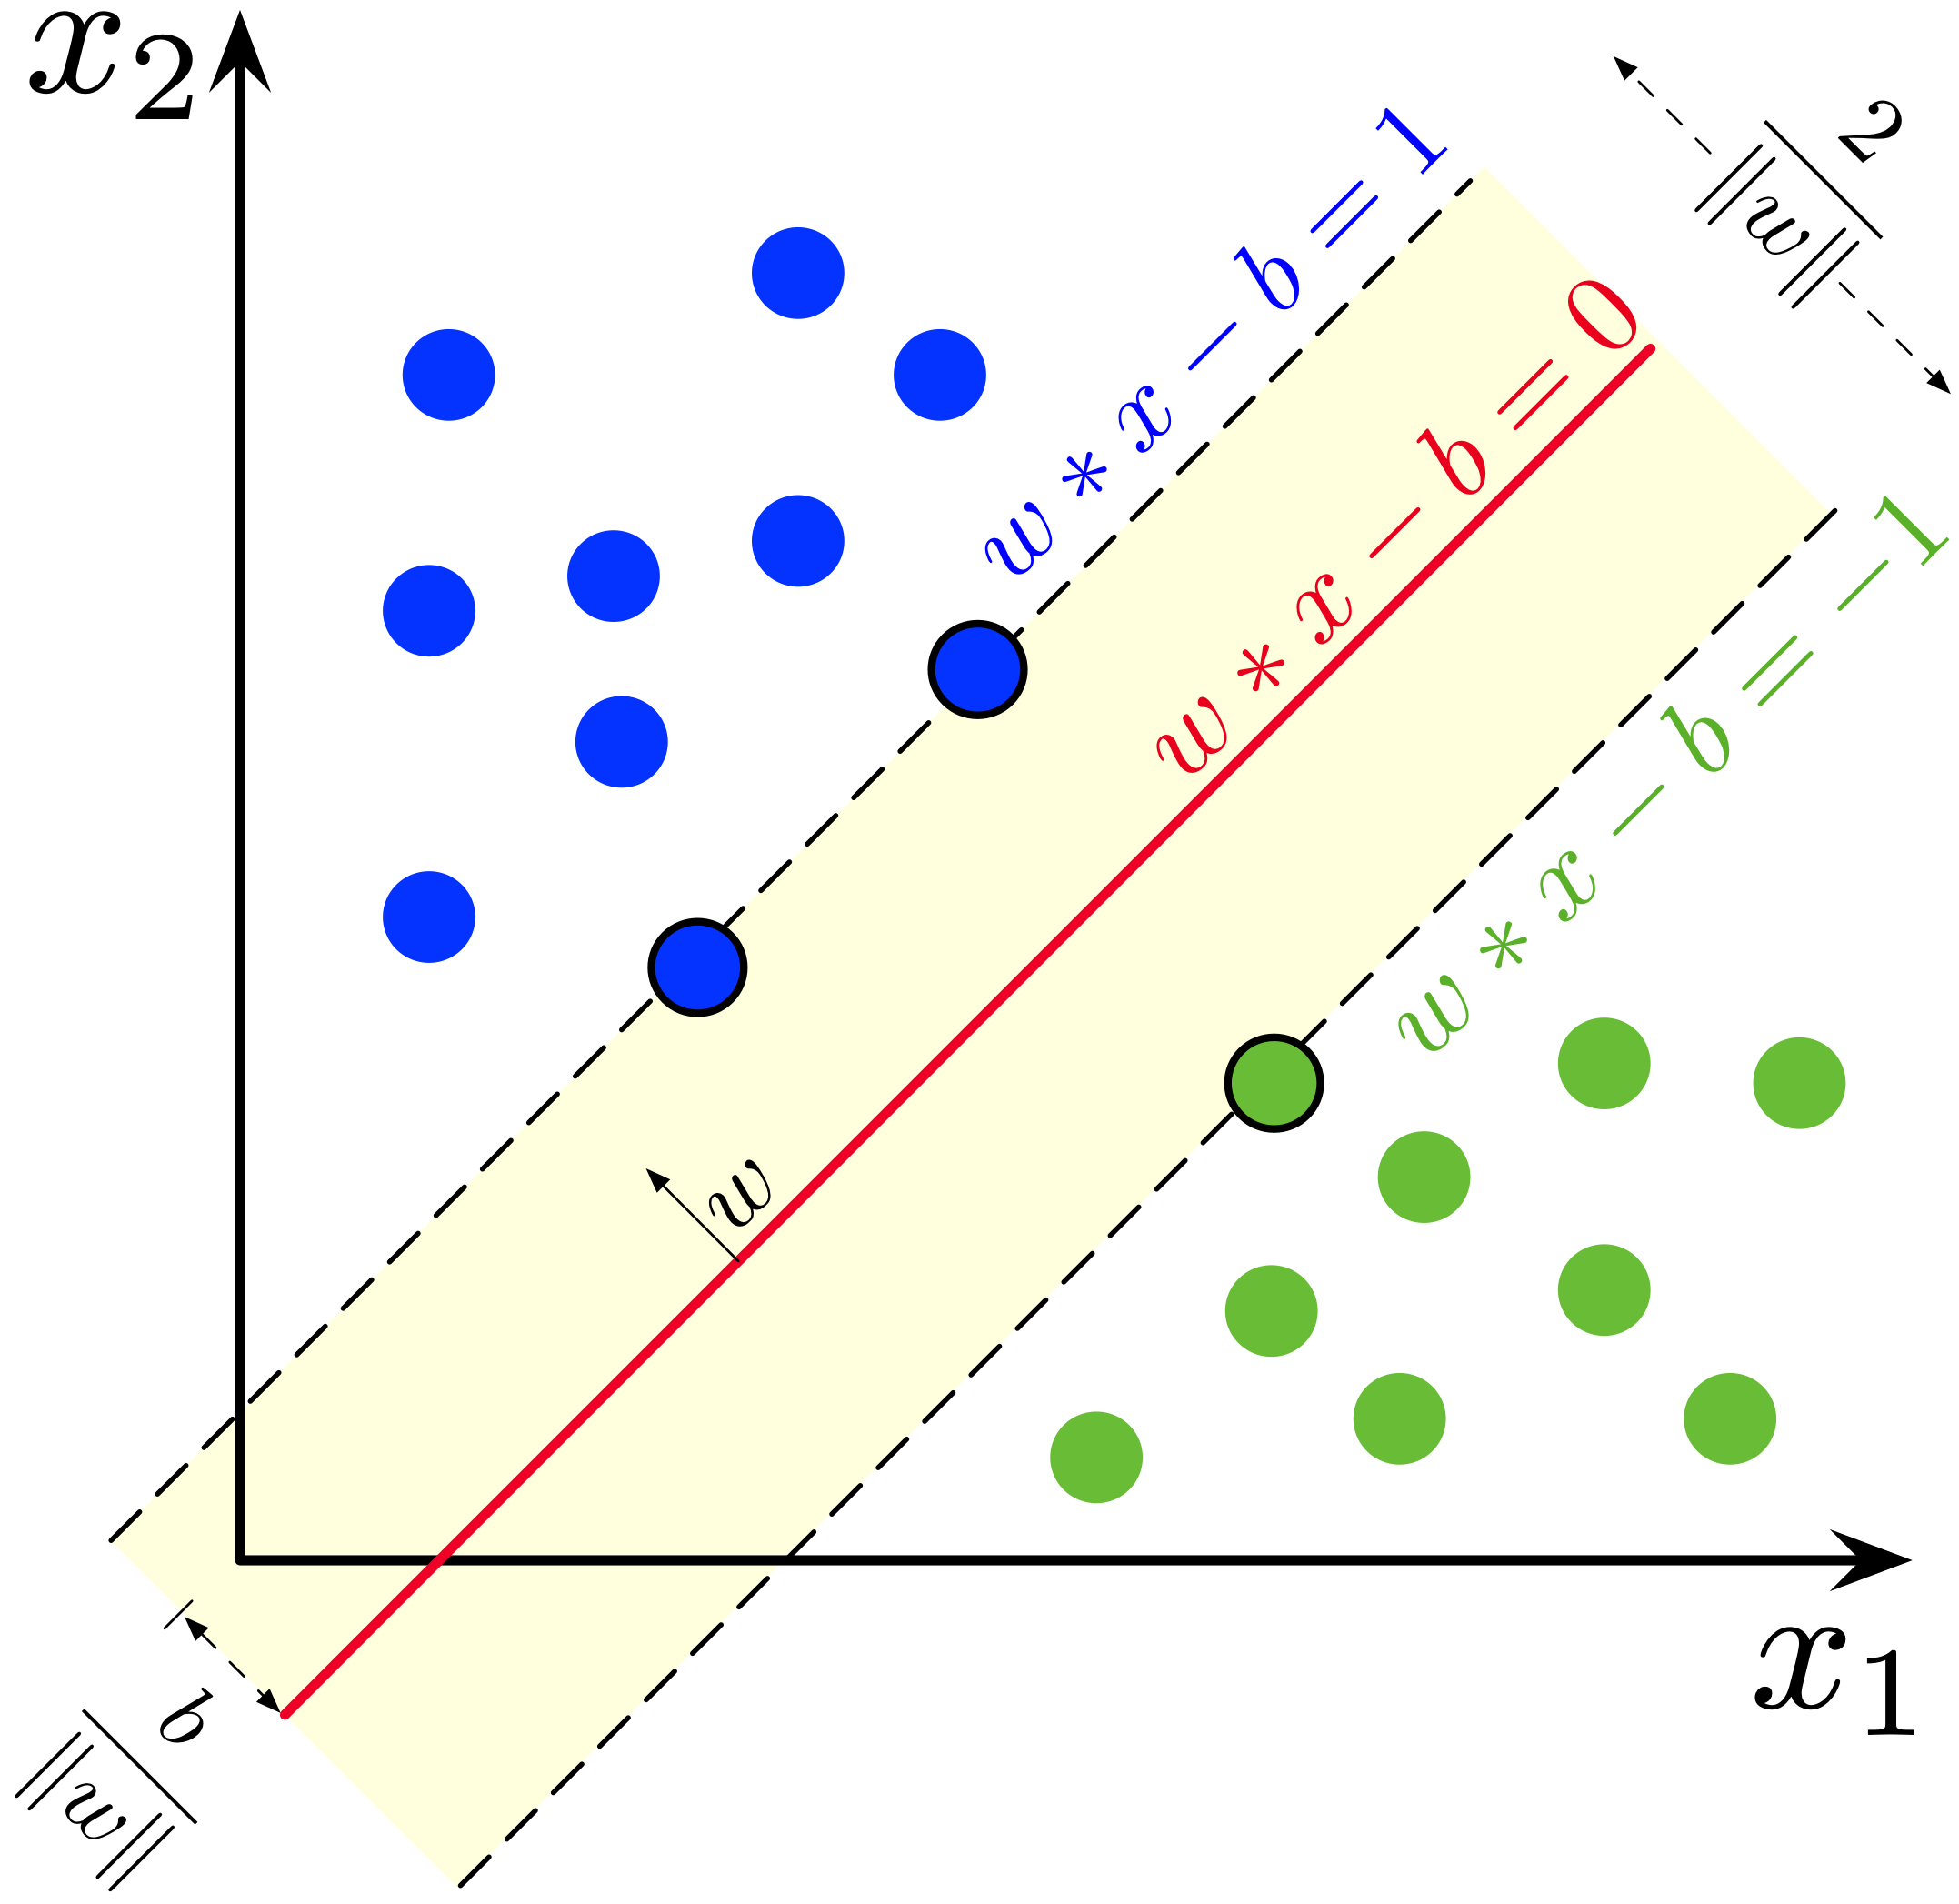
\includegraphics[width=0.5\textwidth]{images/SVM_margin.png}
    \caption{Ejemplo de separación óptima de clases mediante SVM y margen máximo.}
    \label{fig:svm_margin}
\end{figure}

\subsection{Deep Learning}

El \textit{Deep Learning} (aprendizaje profundo) es una subárea del aprendizaje automático que se basa en redes neuronales artificiales con múltiples capas (redes neuronales profundas). Estas redes son capaces de aprender representaciones jerárquicas de los datos, lo que les permite capturar patrones complejos y realizar tareas como clasificación, reconocimiento de imágenes y procesamiento del lenguaje natural.

En el ámbito de los IDS, el \textit{Deep Learning} se utiliza para mejorar la detección de intrusiones mediante la capacidad de aprender características complejas del tráfico de red. Sin embargo, es importante considerar que los modelos de aprendizaje profundo suelen requerir una gran cantidad de datos y recursos computacionales, lo que puede aumentar el consumo energético. Por lo tanto, es crucial buscar enfoques que optimicen el rendimiento sin comprometer la eficiencia energética, alineándose con los principios de la \textit{Green AI}.

\subsubsection{Multilayer Perceptron (MLP)}

El \textbf{Multi-Layer Perceptron} (MLP) es una red neuronal artificial de tipo \textit{feed-forward} compuesta por una capa de entrada, una o varias capas ocultas y una capa de salida. Cada capa está formada por neuronas completamente conectadas, donde cada neurona realiza una combinación lineal de sus entradas seguida de una función de activación no lineal. Este tipo de arquitectura permite aproximar funciones no lineales complejas y es uno de los modelos más utilizados como punto de partida en problemas de aprendizaje profundo.

En el contexto de datasets tabulares, como los empleados en este trabajo, el MLP actúa como un modelo de referencia dentro del aprendizaje profundo, permitiendo evaluar si la introducción de capas no lineales aporta mejoras significativas frente a modelos clásicos como Random Forest o XGBoost. A diferencia de estos últimos, el rendimiento de un MLP depende en gran medida del diseño de la arquitectura y de la correcta selección de hiperparámetros.

Desde el punto de vista computacional, su coste está directamente relacionado con el número de capas ocultas y el número de neuronas por capa. Arquitecturas profundas o excesivamente anchas incrementan de forma notable el tiempo de entrenamiento y el consumo de memoria, sin garantizar necesariamente mejoras en el rendimiento para datos tabulares. Por este motivo, en este trabajo se utilizan arquitecturas MLP compactas, con un número reducido de capas y neuronas, priorizando un equilibrio adecuado entre capacidad de modelado y eficiencia computacional.

En términos de \textit{Green AI}, el MLP representa una alternativa intermedia entre los modelos de aprendizaje automático clásico y redes neuronales más complejas como LSTM o CNN. Aunque su entrenamiento es más costoso que el de modelos basados en árboles, la fase de inferencia sigue siendo relativamente eficiente cuando se emplean arquitecturas ligeras, lo que permite analizar el compromiso entre rendimiento y coste computacional en escenarios de detección de intrusiones.

\begin{table}[H]
    \centering
    \caption{Principales hiperparámetros de MLP y su significado.}
    \label{tab:mlp_hyperparams}
    \begin{tabular}{ll}
        \toprule
        \textbf{Hiperparámetro} & \textbf{Significado} \\
        \midrule
        \texttt{hidden\_layer\_sizes} & Número y tamaño de las capas ocultas \\
        \texttt{activation} & Función de activación utilizada en las neuronas (por ejemplo, \textit{relu}, \textit{tanh}) \\
        \texttt{solver} & Algoritmo de optimización para el entrenamiento (por ejemplo, \textit{adam}, \textit{sgd}) \\
        \texttt{alpha} & Parámetro de regularización L2 \\
        \texttt{learning\_rate\_init} & Tasa de aprendizaje inicial \\
        \texttt{batch\_size} & Tamaño del lote de muestras para cada actualización de los pesos \\
        \texttt{max\_iter} & Número máximo de iteraciones de entrenamiento \\
        \texttt{early\_stopping} & Si se detiene el entrenamiento anticipadamente al no mejorar el rendimiento \\
        \bottomrule
    \end{tabular}
\end{table}

\begin{figure}[H]
    \centering
    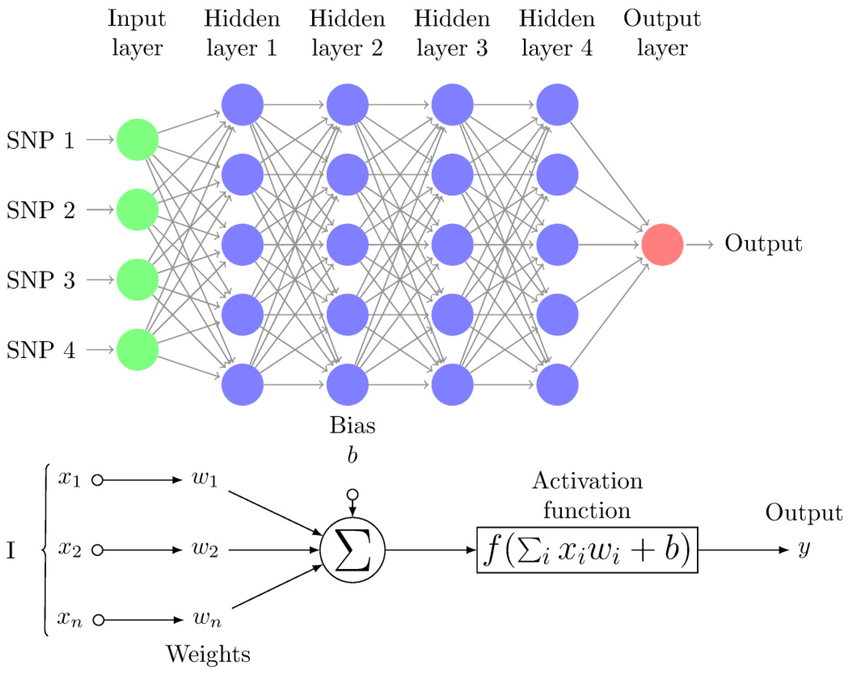
\includegraphics[width=0.7\textwidth]{images/mlp.png}
    \caption{Proceso de retropropagación en una red neuronal MLP.}
    \label{fig:mlp_backpropagation}
\end{figure}

\subsubsection{Long Short-Term Memory (LSTM)}

Las redes \textbf{Long Short-Term Memory} (LSTM) son un tipo de red neuronal recurrente diseñada para modelar dependencias temporales en secuencias de datos. A diferencia de las redes neuronales recurrentes tradicionales, las LSTM incorporan un conjunto de compuertas internas (entrada, olvido y salida) que regulan el flujo de información a lo largo del tiempo, permitiendo conservar o descartar información relevante durante secuencias largas y mitigando el problema del desvanecimiento del gradiente.

En el ámbito de la detección de intrusiones, las LSTM resultan especialmente interesantes cuando el comportamiento malicioso no se manifiesta en observaciones aisladas, sino en patrones temporales que evolucionan a lo largo del tiempo. Aunque los datasets empleados en este trabajo se describen mediante características agregadas a nivel de flujo, el uso de LSTM permite analizar si la introducción de mecanismos de memoria aporta ventajas frente a modelos puramente estáticos, capturando posibles dependencias internas entre características o secuencias de flujos consecutivos.

Desde el punto de vista computacional, las LSTM presentan un coste superior al de modelos \textit{feed-forward} como el MLP, ya que cada unidad recurrente realiza múltiples operaciones internas en cada paso temporal. El número de unidades LSTM y la longitud de las secuencias influyen directamente en el tiempo de entrenamiento y en el consumo de memoria. Por este motivo, en este trabajo se emplean arquitecturas LSTM ligeras, con un número reducido de unidades, evitando configuraciones profundas que resultarían inviables para escenarios con recursos limitados.

En términos de \textit{Green AI}, las LSTM representan un compromiso entre capacidad de modelado y eficiencia. Si bien su entrenamiento e inferencia son más costosos que los de modelos clásicos y MLP sencillos, el uso de configuraciones compactas permite evaluar de forma controlada el impacto de la modelización temporal en el rendimiento del sistema IDS. De este modo, las LSTM se incluyen como un modelo de referencia para analizar el beneficio potencial de incorporar memoria temporal frente al incremento del coste computacional asociado.

\begin{table}[H]
    \centering
    \caption{Principales hiperparámetros de LSTM y su significado.}
    \label{tab:lstm_hyperparams}
    \begin{tabular}{ll}
        \toprule
        \textbf{Hiperparámetro} & \textbf{Significado} \\
        \midrule
        \texttt{units} & Número de unidades LSTM en la capa recurrente \\
        \texttt{return\_sequences} & Si la capa devuelve la secuencia completa o solo el último estado \\
        \texttt{dropout} & Tasa de abandono para regularización durante el entrenamiento \\
        \texttt{recurrent\_dropout} & Tasa de abandono aplicada a las conexiones recurrentes \\
        \texttt{activation} & Función de activación utilizada en las unidades LSTM (por ejemplo, \textit{tanh}) \\
        \texttt{recurrent\_activation} & Función de activación para las compuertas internas (por ejemplo, \textit{sigmoid}) \\
        \texttt{learning\_rate\_init} & Tasa de aprendizaje inicial para el optimizador \\
        \texttt{batch\_size} & Tamaño del lote de muestras para cada actualización de los pesos \\
        \texttt{max\_iter} & Número máximo de iteraciones de entrenamiento \\
        \bottomrule
    \end{tabular}
\end{table}

\begin{figure}[H]
    \centering
    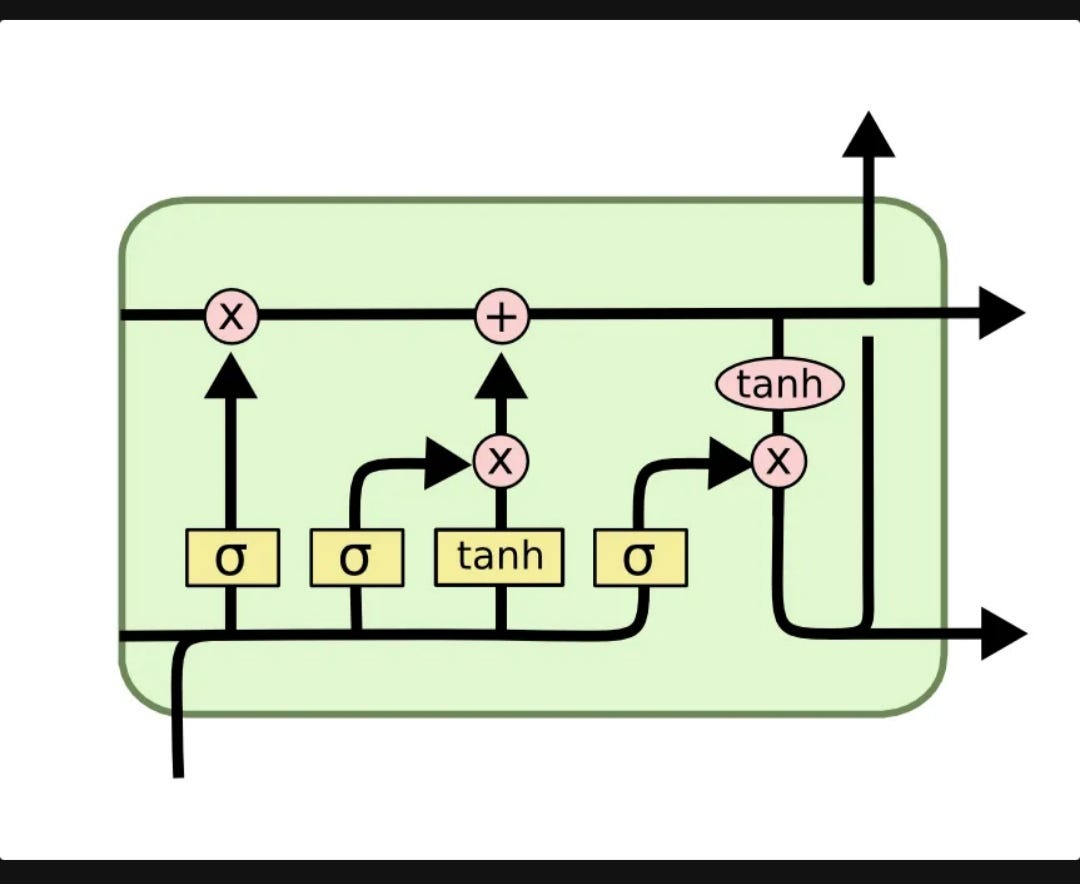
\includegraphics[width=0.45\textwidth,clip,trim=0cm 1.2cm 0cm 1.2cm]{images/lstm.jpg}
    \caption{Esquema representativo de una unidad LSTM con sus compuertas internas.}
    \label{fig:lstm_unit}
\end{figure}


\subsubsection{Convolutional Neural Networks (CNN)}

Las \textbf{Convolutional Neural Networks} (CNN) son un tipo de red neuronal profunda diseñadas originalmente para el procesamiento de datos con estructura espacial, como imágenes o señales. Su principal característica es el uso de capas convolucionales, que aplican filtros locales sobre los datos de entrada para extraer patrones relevantes de forma jerárquica, reduciendo al mismo tiempo el número de parámetros respecto a redes completamente conectadas.

En el contexto de este trabajo, las CNN se emplean en su variante \textit{1D}, donde las convoluciones se aplican sobre el vector de características de cada flujo de red, tratado como una señal unidimensional. Este enfoque permite capturar relaciones locales entre características adyacentes, modelando interacciones de corto alcance entre variables sin necesidad de introducir arquitecturas excesivamente complejas. De este modo, la CNN 1D actúa como una alternativa intermedia entre el MLP y las redes recurrentes, explorando si la extracción local de patrones aporta mejoras en la detección de intrusiones.

Desde el punto de vista computacional, el coste de una CNN depende principalmente del número de filtros, el tamaño del kernel y la profundidad de la red. Aunque las CNN suelen ser más eficientes que otras arquitecturas profundas al compartir pesos, un número elevado de filtros o capas puede incrementar significativamente el tiempo de entrenamiento y la latencia de inferencia. Por esta razón, en este trabajo se utilizan arquitecturas CNN poco profundas y con un número reducido de filtros, priorizando configuraciones compactas y eficientes.

En términos de \textit{Green AI}, la CNN 1D representa un compromiso entre capacidad de representación y eficiencia computacional. Si bien su coste es superior al de modelos clásicos y MLP sencillos, una arquitectura cuidadosamente limitada permite evaluar el impacto de la extracción convolucional de patrones manteniendo un consumo de recursos razonable.

\begin{table}[H]
    \centering
    \caption{Principales hiperparámetros de CNN y su significado.}
    \label{tab:cnn_hyperparams}
    \begin{tabular}{ll}
        \toprule
        \textbf{Hiperparámetro} & \textbf{Significado} \\
        \midrule
        \texttt{filters} & Número de filtros en la capa convolucional \\
        \texttt{kernel\_size} & Tamaño del kernel de convolución (por ejemplo, 3) \\
        \texttt{strides} & Paso de la convolución sobre la entrada \\
        \texttt{padding} & Tipo de relleno aplicado a los bordes (por ejemplo, \textit{same}, \textit{valid}) \\
        \texttt{activation} & Función de activación utilizada en las capas convolucionales (por ejemplo, \textit{relu}) \\
        \texttt{learning\_rate\_init} & Tasa de aprendizaje inicial para el optimizador \\
        \texttt{batch\_size} & Tamaño del lote de muestras para cada actualización de los pesos \\
        \texttt{max\_iter} & Número máximo de iteraciones de entrenamiento \\
        \bottomrule
    \end{tabular}
\end{table}

\begin{figure}[H]
    \centering
    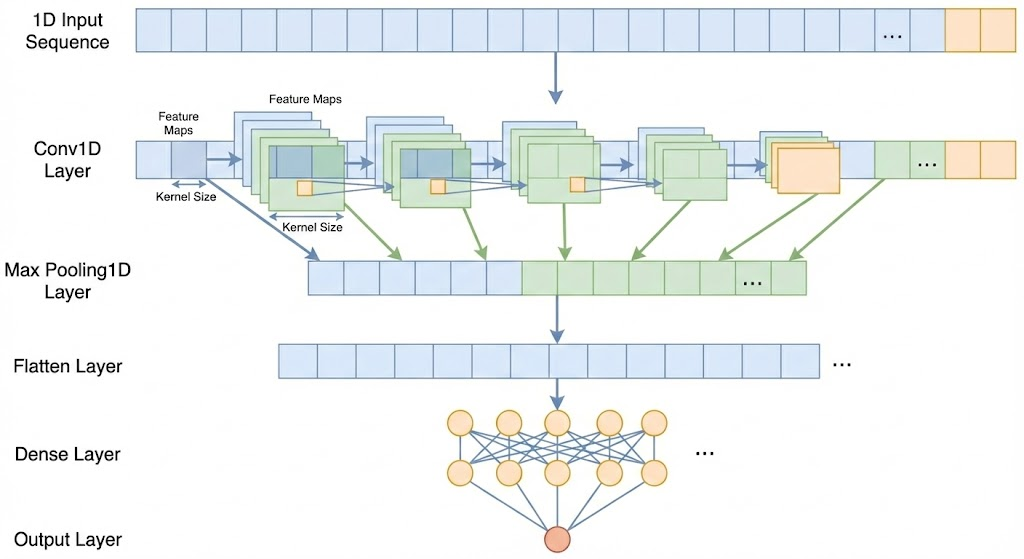
\includegraphics[width=0.7\textwidth]{images/CNN_1D.jpg}
    \caption{Esquema representativo de una arquitectura CNN 1D aplicada a datos tabulares.}
    \label{fig:cnn_1d}
\end{figure}

